%\section{PILOT STUDY}
%Owing to natural bio-mechanism of human hands, using the index fingertips as  touchpads confronts unique usability concerns. %is not as easy as conventional touch pads.
%Firstly, unlike flat touch pads, fingertips are soft and curve, causing regions in the index fingertip not equally reachable by the thumb. Secondly, unlike touchpads, the motor space in the index and the thumb fingertips (i.e., the pad and the stylus) are constrained because they are mechanically connected by joints. 

%inter-connected, due to motor space of the two fingers is constrained due to the fact that the index and thumb are mechanically connected by joints. %Both make the touch regions in index fingertips not equally attainable.
%visible by the user eyesights and 

%To understand how to design touch interface for finger pads, we conducted a pilot study to determine the comfort levels in fingertip regions, as shown in Figure \ref{fig:pilotStudy}. 

%The participant was instructed to tap on regions in the index fingertip using the thumb tip. 
%To control the touch positions across participants, we stick thin translucent dot pattens  of their size (Figure \ref{fig:pilotStudy}a) on their index fingertips. 

%We divided the index fingertip into a 4 by 4 grid; each cell was represented by a dot. In task 1, the participants pressed the dots (three repetitions each cell, randomized) indicated on the screen. In task 2, they wrote a series of numbers on the fingertip. Participants performed the task without looking at their input fingers.

%The 4 by 4 dots evenly arranged across the fingertip. 
%, wrote a series of numbers on the fingertip (Figure \ref{fig:pilotStudy}c), and ranked comfort levels in the regions suggested by dots. %guide the participants the touch positions

%There were two tasks. In the first task, the participants pressed the dots indicated on the screen (Figure \ref{fig:pilotStudy}b), and wrote a series of numbers on the fingertip (Figure \ref{fig:pilotStudy}c). In the second task, we played an animation in which a cursor moved over a button and committed the selection. The participants emulate the effect  by performance using the pinched fingertips. A questionnaire followed up the study.

%\begin{figure}
%\begin{center}
%  \begin{tabular}{@{\hspace{0.1cm}}c}
%		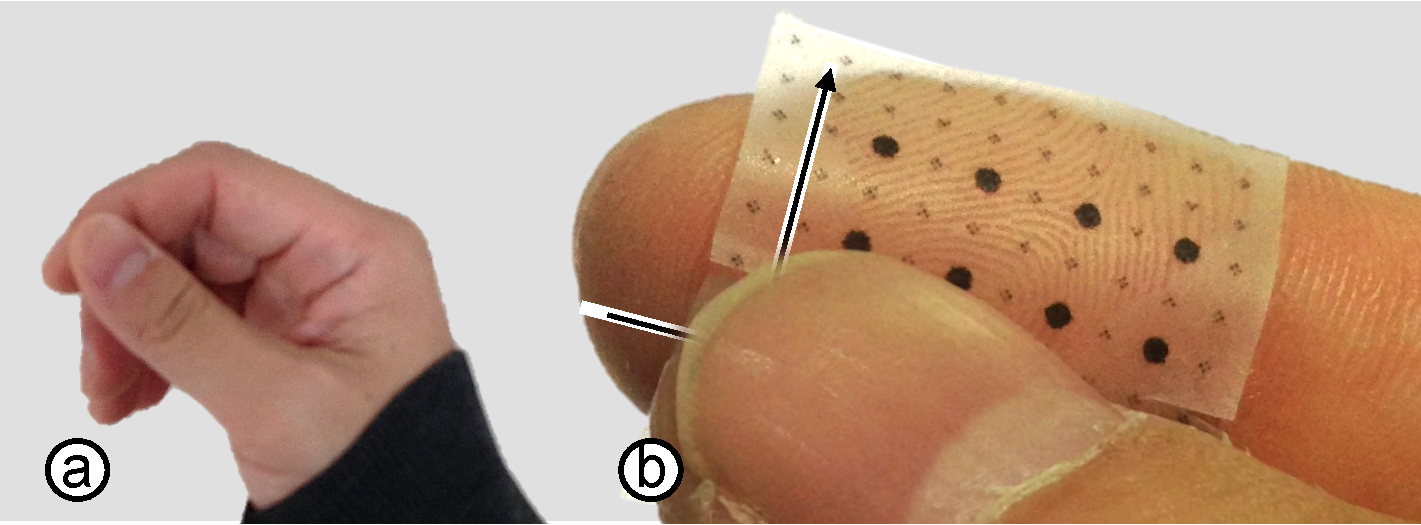
\includegraphics[width=1\linewidth]{pilotStudy}
%   \end{tabular}
%\caption{(a) The posture the participants were instructed to perform in the pilot study. (b) The translucent dot pattern stick on the fingertip to guide the participants through touch.}
%\label{fig:pilotStudy}
%\end{center}
%\end{figure}

%\begin{figure}
%\begin{center}
%  \begin{tabular}{@{\hspace{0.1cm}}c}
%		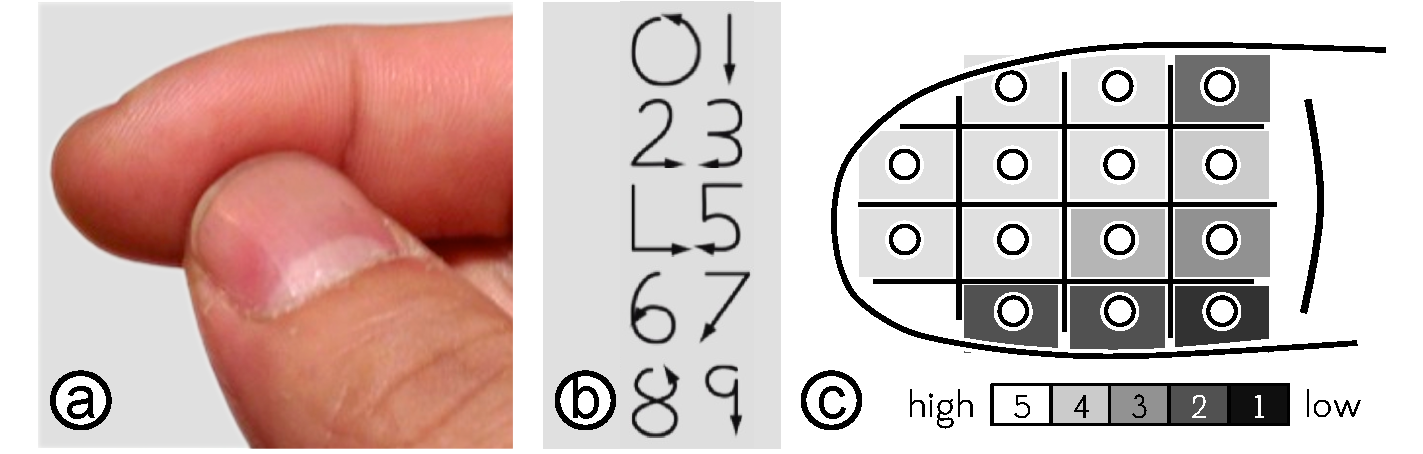
\includegraphics[width=1\linewidth]{pilotStudy5}
%   \end{tabular}
%\caption{(a) The pilot study includes two tasks: (a) the tapping task and (b) the drawing task. (c) Participants rank comfort levels of touch in the regions across the index fingertip.}
%\label{fig:pilotStudy}
%\end{center}
%\end{figure}

%\subsection{Result \& discussion}
%7 participants (3 females), between 22 and 34, were recruited, all right-handed. 2 female participants had long nails.
%Figure \ref{fig:pilotStudy}c shows the average comfort levels across regions in the index fingertip. Brighter region indicates higher comfort level.
%The result reported that the inner regions (lower-right regions) in the index fingertips in general received lower comfort levels than the outer regions. 
%The participants who had this tendency described that it required additional force to bend thumb limbs in order to reach the dots at the bottom row and, in particular, the dot at bottom-right corner.

%\subsubsection{Bent or hunched postures}
%We found two primary types of thumb-as-stylus postures that affected the comfort levels. 
%The participants either (a) bent the thumb (Figure \ref{fig:twoTypesOfThumb}a) such that the thumb tip pointed from below the index fingertip, or (b) hunched the thumb (Figure \ref{fig:twoTypesOfThumb}b), allowing to point from above.
%The participants (3 out of 7) who applied bent postures gave 2.3 times lower in comfort levels at regions in the bottom row than the participants who applied hunched postures. With further instructions, all but one participants, who used the bent postures at trials, reported they can use the hunched posture without problems. 

%We also asked how they determined the touch positions through haptics. 
%In the regions easier reachable (e.g., the outer regions), participants with short nails determined the touch through the contact area close to the edge of the thumb tip, similar to the projection model suggested by Christian Holz \cite{Holz:2011}. This strategy switched to using sharp haptics through the nail edge, when their thumbs had extended nails.
%Two female participants who had long nails touched the bottom row regions using the nail back (\ref{fig:fingerpadFunction}a), which, to a large extent, degraded their sense of touch positions.

%\subsection{Touch Interface Design}
%As illustrated by Figure \ref{fig:fingerpadFunction}b, we divide the index fingertip into two functional regions: the pad and the bezel regions. The pad region covers the central and upper parts of the fingertip, suggesting a near flat and easily reachable area.
%In the bezel region, we install a big button on the bottom, and a button on the very end of index fingertip. The bezel buttons allow short cut operations, such as the \textit{home button} illustrated by Figure \ref{fig:walkthrough}g in the \textit{SCENARIO}.

%In \ref{fig:twoTypesOfThumb}a, the participants bent the thumb downward such that the thumb tip pointed from below the index fingertip. In \ref{fig:twoTypesOfThumb}b, the participants hunched up the thumb such that the thumb tip pointed from above. 

%\subsubsection{Friction}

%\subsubsection{Area of comfort}

%\begin{figure}
%\begin{center}
%  \begin{tabular}{@{\hspace{0.1cm}}c}
%		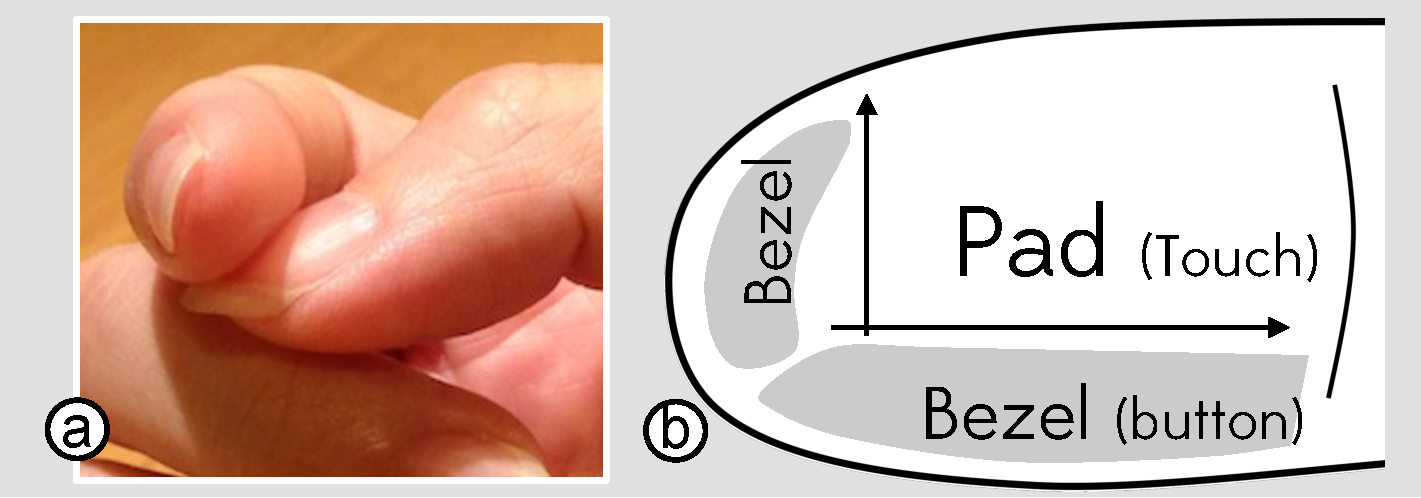
\includegraphics[width=1\linewidth]{fingerpadFunction8}\\
%   \end{tabular}
%\caption{(a) The participant with long nail touched the bottom regions with the nail back. (b) According to the pilot study, we divide the index fingertip into two functional regions: the pad and the bezel regions, for touch pad input and button input. }
%\label{fig:fingerpadFunction}
%\end{center}
%\end{figure}




%\subsubsection{commitment method}

%\subsubsection{Activation}



%\begin{figure}
%\begin{center}
%  \begin{tabular}{@{\hspace{0.1cm}}c}
%		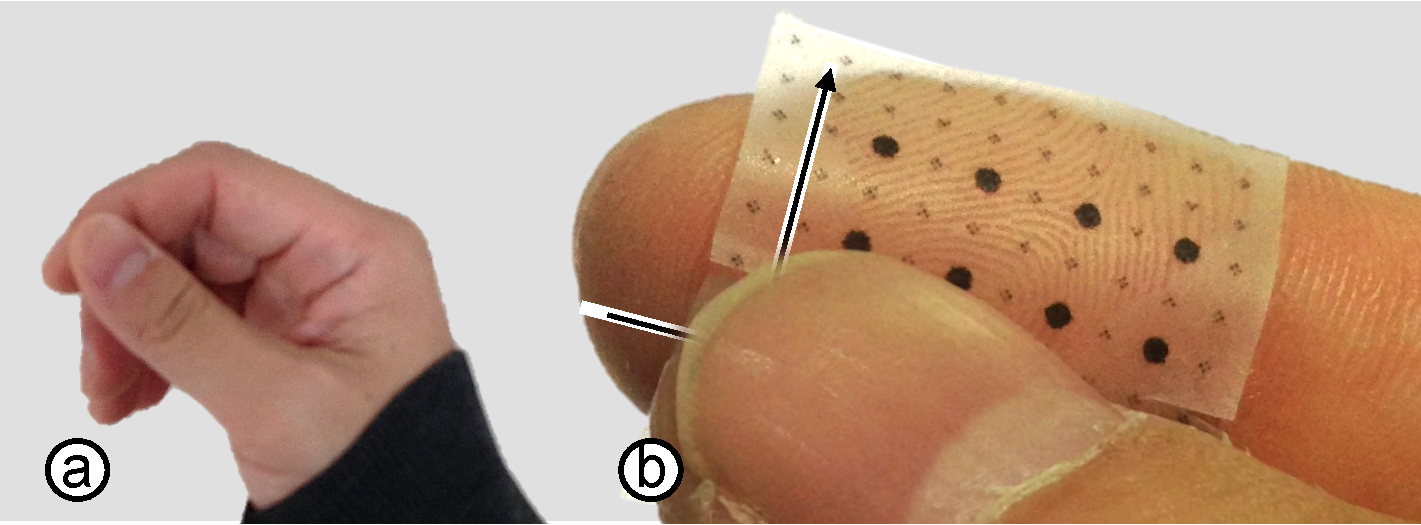
\includegraphics[width=1\linewidth]{pilotStudy}\\
%   \end{tabular}
%\caption{(a) The posture the participants were instructed to perform in the pilot study. (b) The translucent dot pattern stick on the fingertip to guide the participants through touch.}
%\label{fig:pilotStudy}
%\end{center}
%\end{figure}


%\section{DESIGN: IndexPad v.s. ThumbPad}
%Unlike touchpads where the finger is always considered as an input pen, FingerPad's  pad and pen, referring to index and thumb fingertips, are interchangeable. We include two models into consideration: IndexPad and ThumbPad, depending on which fingertip users perceive as the finger touchpad. Misinterpretation of the model applied can lead to inverted results. For example, on a finger pinch, the sense of touch is contributed from the contact regions locating at different parts in the index and thumb fingertips. These regions suggest different touch positions in both fingertips, as well as in the user's mental. Unfortunately, the model applied only exists in users head. Without understanding what might trigger the decision of the model to use, interaction with FingerPad can be frustrating. 

%To understand how users determine which model to use, and what pros and cons each model inherits, we conduct a pilot study.

%We argue that  this decision is affected by the orientations of the fingertips. Unlike touchpads which always face up allowing for touch, the orientation of FingerPad can be various depending on the context of use. The fact that wearing input devices on fingertips suggests using the device instantly at anytime, as shown in Figure \ref{fingerPadPosture}, making this worse.

%Moreover, unlike touchpads which always face up allowing for touch, the orientation of FingerPad can be various depending on the context of use. 
%Depending on the context of use, FingerPad's orientation can be various yet unexpected. 
%The key seems to understand  when and why users perceived their fingertips as the pads.
%Moreover, the fact that wearing input devices on fingertips suggest using it instantly at anytime makes this worse.
%FingerPad allows two distinct interpretations of touch. 

%\label{fig:typeOfPads}

%\subsection{Functional regions}
%Center and upper area receive good comfort level in touch. Lower part is not easily seen. Very lower part often tapping with nail back. Left part taping with thumb tip side. Show several examples in Figure \ref{fig:functionRegion}a.

%As suggesting by the results, we divide the index fingertip into two functional regions: the touch pad , and the bezel buttons, as shown in Figure \ref{fig:functionRegion}b. The pad region suggests a flat surface that maximize visibility and facilitate touch behavior. The bezel regions, on the tip and lower part of the index fingertip, allows buttons to e.g., invoke menus. While the lower part seems wide enough to embed more buttons, we simplify it to single big button because the comfort level is low and the way users might touch it is versatile.

%\begin{figure}
%\begin{center}
%  \begin{tabular}{@{\hspace{0.1cm}}c}
%		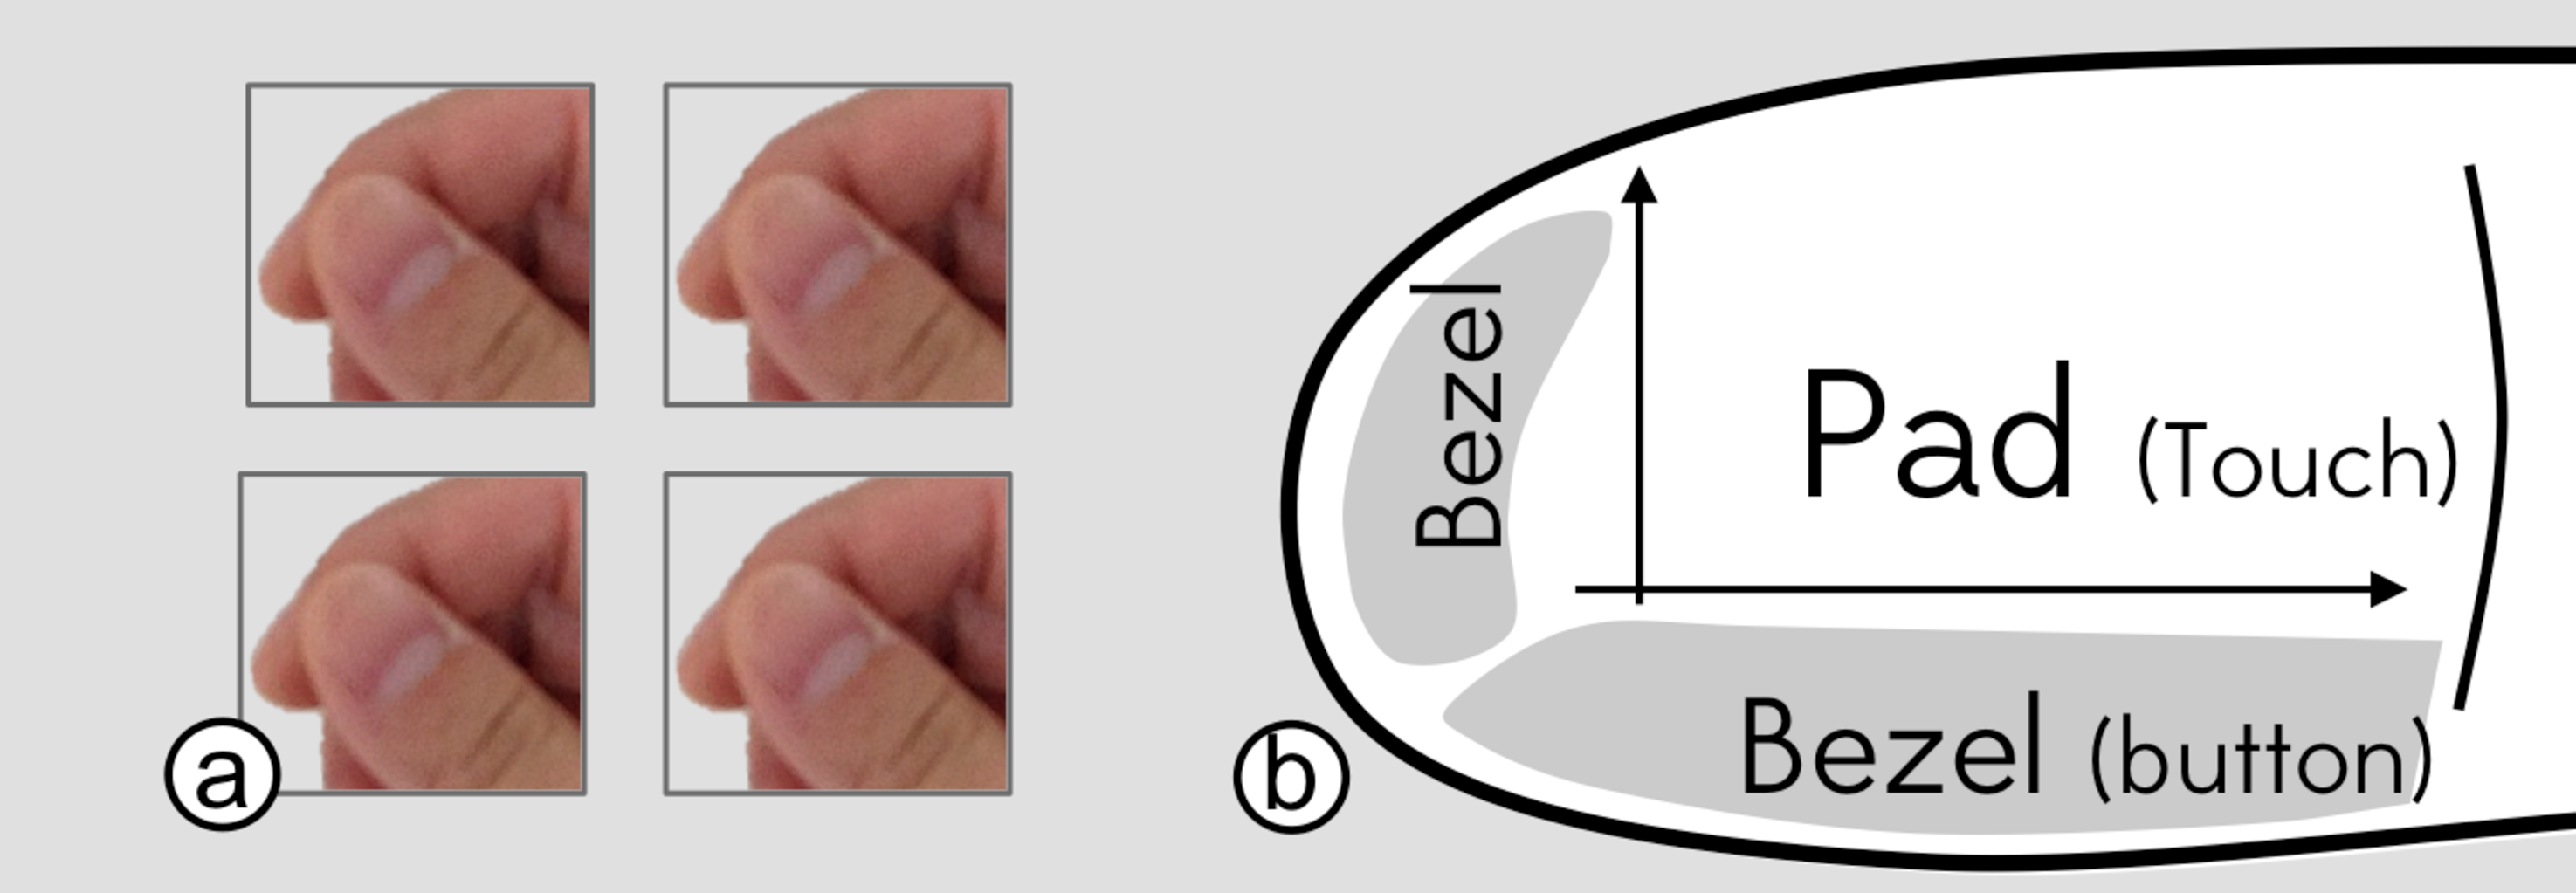
\includegraphics[width=1\linewidth]{fingerpadFunction7}\\
%   \end{tabular}
%\caption{(a) Example postures of the thumb tapping at tip and lower part of the index fingertip. (b)Design of functional regions in FingerPad.}
%\label{fig:functionRegion}
%\end{center}
%\end{figure}
